\chapter{Antipodal double covers of regular graphs}
\label{4classbip}
\section{Intro -- Will be removed, only here as a marker}

\section{Projective doubles of regular graphs}

Let $\Gamma$ be an undirected graph on $v$ vertices. A \emph{projective double} of $\Gamma$ is an antipodal (spherical) $4$-distance set, say $L = \left\{\ell_1,\dots,\ell_{2v}\right\}$ with inner products $A = \left\{1,\alpha,0,-\alpha,-1\right\}$, such that there exists a mapping $\phi:L\rightarrow V\Gamma$ fulfilling
\begin{enumerate}[label=(\roman*)]
	\item $\phi(\ell_i) = \phi(\ell_j)$ if and only if $\left\vert\left<\ell_i,\ell_j\right>\right\vert = 1$,
	\item $\phi(\ell_i) \sim \phi(\ell_j)$ if and only if $\left\vert\left<\ell_i,\ell_j\right>\right\vert = \alpha$
\end{enumerate}
for $1\leq i,j\leq 2v$. Since the inner products are determined by a single parameter $\alpha$, we will often say $L$ is a projective double of $\Gamma$ with inner product $\alpha$. Note that $(ii)$ implies that for vertices $v,w\in V\Gamma$, $v\not\sim w$ implies $\phi^{-1}(v)$ and $\phi^{-1}(w)$ are orthogonal sets. We initially consider when such projective doubles may exist, however this ends up being uninteresting if we allow our dimension to be large enough.
\begin{prop}\label{dirnaive}
	For any non-empty simple graph $\Gamma$, there exists a projective double in $\mathbb{R}^{m}$ for some $m\leq \vert V\Gamma\vert$ with $\alpha = d^{-1}$ with $d$ the max degree of $\Gamma$.
\end{prop}
\begin{proof}
	Let $\Gamma = \Gamma(V,E)$ be given. Now orient every edge of $\Gamma$ and define $e_i^+,e_i^-\in V$ so that $e_i = (e_i^-,e_i^+)$, thus $e_i$ points from vertex $e_i^-$ to $e_i^+$. Let $M$ be the matrix with rows indexed by vertices and columns indexed by edges such that
	\[\left[M\right]_{ij} =\begin{cases} 1 &\text{ if }v_i = e_j^+\\
	-1 &\text{ if }v_i = e_j^-\\
	0 &\text{ otherwise. }
	\end{cases}\]
	Then we find 
	\[\left[MM^T\right]_{ij} = \begin{cases}
	k_i & \text{ if }i=j,\\
	1 & \text{ if } i\sim j,\\
	0 & \text{ otherwise}
	\end{cases}\]
	where $k_i$ is the degree of vertex $i$. Thus two distinct rows are orthogonal if and only if their corresponding vertices are non-adjacent. However unless $k_i$ is constant independent of $i$ (the graph is regular), the rows do not have the same norm. To solve this, let $d = \max_{i}(k_i)$ (the max degree of $\Gamma$) and define the diagonal matrix $D$ whose $i^\text{th}$ diagonal entry is $\sqrt{d-k_i}$. Then the matrix $N = \left[\begin{array}{c|c}
	M & D
	\end{array}\right]$ has the property that
	\[\left[NN^T\right]_{ij} = \left[MM^T\right]_{ij} + (k-k_i)\delta_{ij} = \begin{cases}
	d & \text{ if }i=j,\\
	1 & \text{ if } i\sim j,\\
	0 & \text{ otherwise.}
	\end{cases}\]
	Thus the rows of $\frac{1}{\sqrt{d}}N$, along with their negatives, result in a projective double of $\Gamma$ with inner product $\frac{1}{d}$. Further the rank of $N$ is no larger than $\max\left\{\vert V\vert, \vert V\vert+\vert E\vert\right\} = \vert V\vert$.
\end{proof}
\begin{cor}\label{regnaive}
	For any regular graph $\Gamma$ with at least one edge, there exists a projective double in $\mathbb{R}^m$ with inner product $\frac{1}{k}$ for some $m\leq T$ where $k$ is the regularity and $T$ is the number of edges in any spanning forest.
\end{cor}
\begin{proof}
	We follow the same proof as with Proposition \ref{dirnaive} however we note that since our graph is regular and non-empty, the rows of $M$ with their negatives all have the same norm. Thus the normalized rows suffice to serve as our projective double with inner product $\frac{1}{k}$. In this case, we have immediately that $\rank(M) \leq \text{min}\left\{\vert V\vert,\vert E\vert\right\}$. However, consider any cycle $C$ in our graph and assume without loss of generality that $C = \left\{e_1,\dots,e_s\right\}$. Then, replacing a column with its negative if necessary, $\displaystyle{M_{e_s} = \sum_{i=1}^{s-1}M_{e_{i}}}$ and thus these columns are linearly dependent. Then reorder the columns of $M$ so that the first $T$ edges correspond to the edges of a spanning forest. Including any column after these $T$ columns results in a linearly dependent set of columns, forcing $\text{rank}(M) \leq \text{min}\left\{\vert V\vert,T\right\}$. Further, for any nonempty regular graph, $\vert T\vert\leq \vert V\vert$ and therefore $\text{rank}(M) \leq T$
\end{proof}
Proposition \ref{dirnaive} and corollary \ref{regnaive} provide upper bounds on the dimension necessary for a projective double to exist for a given graph. The following observation gives us a lower bound using the independence number of a graph $\alpha\left(\Gamma\right)$. That is, $\alpha\left(\Gamma\right)$ is the largest set of vertices in $\Gamma$ which are pairwise non-adjacent.
\begin{prop}\label{cocliquebnd}
	Let $\Gamma$ be a simple graph and $L$ be a projective double of $\Gamma$ in $\mathbb{R}^m$. Then $m\geq \alpha\left(\Gamma\right)$ where $\alpha\left(\Gamma\right)$ is the independence number of $\Gamma$.
\end{prop}
\begin{proof}
	Assume we have a projective double of $\Gamma$ in $\mathbb{R}^m$ with $\phi(\pm\ell_i) = v_i$ for $1\leq i\leq\vert V\vert$. Let $\alpha = \alpha\left(\Gamma\right)$ and without loss of generality let $S = \left\{v_1,\dots,v_\alpha\right\}$ be an independent set. Then $\left\{\ell_1,\dots,\ell_\alpha\right\}$ is an orthonormal set, forcing $m\geq\alpha$.
\end{proof}
We are interested in when we may achieve this lower bound.
\begin{example}\label{doublecoverc4}
Consider the graph $C_4$. This is a regular graph with 3 edges in any spanning tree, thus Corollary \ref{regnaive} tells us there exists a projective double in $\mathbb{R}^3$ with inner product $\frac{1}{2}$. In fact, the columns of $U_1$ serve as one such projective double with $\alpha = \frac{1}{2}$. 
\[U_1 = \left[\begin{array}{crcccccc}
1 & -1 & \frac{1}{2} & -\frac{1}{2} & 0 & 0 &\frac{1}{2} &-\frac{1}{2}\\
0 & 0 & \frac{\sqrt{3}}{2} & -\frac{\sqrt{3}}{2} & \frac{1}{\sqrt{3}} & -\frac{1}{\sqrt{3}} & -\frac{1}{\sqrt{12}}& \frac{1}{\sqrt{12}}\\
0 & 0 & 0 & 0 & \sqrt{\frac{2}{3}} & -\sqrt{\frac{2}{3}} & \sqrt{\frac{2}{3}} & -\sqrt{\frac{2}{3}} \\			
\end{array}\right]\]
However, the maximum independent set in this graph has size $2$ and thus Proposition \ref{cocliquebnd} allows for the possibility of a projective double in $\mathbb{R}^2$. While it is not hard to show that we cannot find a projective double in $\mathbb{R}^2$ with inner product $\frac{1}{2}$, we may change the inner product to $\frac{1}{\sqrt{2}}$ and find an example. In fact, the columns of $U_2$ give us exactly that.
\[U_2 = \left[\begin{array}{crcrcccc}
1 & -1 & 0 & 0 & \frac{\sqrt{2}}{2} & -\frac{\sqrt{2}}{2} & \frac{\sqrt{2}}{2} & -\frac{\sqrt{2}}{2}\\
0 & 0 & 1 & -1 & \frac{\sqrt{2}}{2} & -\frac{\sqrt{2}}{2} & -\frac{\sqrt{2}}{2} & \frac{\sqrt{2}}{2}\\				
\end{array}\right]\]
To see the difference between $U_1$ and $U_2$, consider the graph $\Gamma_\alpha(L,E)$ with $(\ell_i,\ell_j)\in E$ if and only if $\left<\ell_i,\ell_j\right> = \alpha$. Using the columns of $U_1$ as our projective double, we find that $\Gamma_{\frac{1}{2}}$ is given below where $v_i$ represents the $i^\text{th}$ column of $U_1$.
\[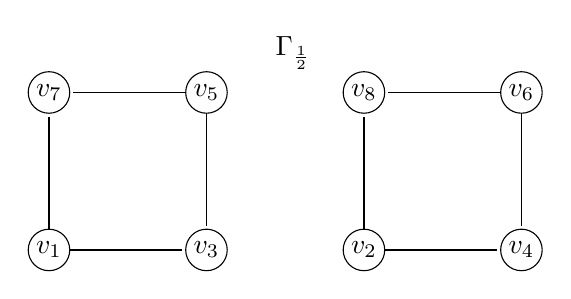
\begin{tikzpicture}[shorten >=1pt,auto,node distance=2cm,
thin,main node/.style = {circle,draw, inner sep = 0pt, minimum size = 15pt}]

\node[main node,fill=white] (1) {$v_1$};
\node[main node,fill=white] [right of = 1](2) {$v_3$};
\node[main node,fill=white] [above of = 1](3) {$v_7$};
\node[main node,fill=white] [above of =2](4) {$v_5$};
\node[main node,fill=white] [right of =2](5) {$v_2$};
\node[main node,fill=white] [right of = 5](6) {$v_4$};
\node[main node,fill=white] [above of = 5](7) {$v_8$};
\node[main node,fill=white] [above of =6](8) {$v_6$};
\node at (3.1,2.5) (9) {$\Gamma_{\frac{1}{2}}$};

\path[-]
(1) edge node {} (2)
edge node {} (3)
(4) edge node {} (3)
edge node {} (2)
(5) edge node {} (6)
edge node {} (7)
(8) edge node {} (7)
edge node {} (6);
\end{tikzpicture}\]
However if we instead consider $U_2$ as our projective design, $\Gamma_{\frac{\sqrt{2}}{2}}$ is given by
\[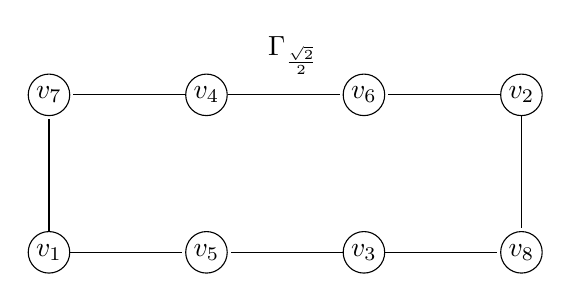
\begin{tikzpicture}[shorten >=1pt,auto,node distance=2cm,
	thin,main node/.style = {circle,draw, inner sep = 0pt, minimum size = 15pt}]
	
	\node[main node,fill=white] (1) {$v_1$};
	\node[main node,fill=white] [right of = 1](2) {$v_5$};
	\node[main node,fill=white] [above of = 1](3) {$v_7$};
	\node[main node,fill=white] [above of =2](4) {$v_4$};
	
	\node[main node,fill=white] [right of =2](5) {$v_3$};
	\node[main node,fill=white] [right of = 5](6) {$v_8$};
	\node[main node,fill=white] [above of = 5](7) {$v_6$};
	\node[main node,fill=white] [above of =6](8) {$v_2$};
	\node at (3.1,2.5) (9) {$\Gamma_{\frac{\sqrt{2}}{2}}$};
	
	\path[-]
	(1) edge node {} (2)
	edge node {} (3)
	(4) edge node {} (3)
	edge node {} (7)
	(5) edge node {} (6)
	edge node {} (2)
	(8) edge node {} (7)
	edge node {} (6);
\end{tikzpicture}\]
Thus $U_1$ and $U_2$ are non-isomorphic as their corresponding graphs are non-isomorphic double covers of $C_4$. Even further, define the five relations $R_0,\dots,R_4$ via the inner products $1$, $\alpha$, $0$, $-\alpha$, and $-1$ respectively so that, for instance, $(x,y)\in R_2$ if and only if the corresponding vectors are orthogonal. These four relations satisfy all the requirements of an association scheme except for possibly the existence of intersection numbers. In the case of the projective double $U_1$, we find that $p^2_{11}$ is not well defined;
\[\left\vert\left\{v_x : (v_x,v_1),(v_5,v_x)\in R_{\alpha}\right\}\right\vert\neq\left\vert\left\{v_x : (v_x,v_1),(v_4,v_x)\in R_{\alpha}\right\}\right\vert\]
yet $(v_1,v_4),(v_1,v_5)\in R_{2}$. However the projective double $U_2$ has well-defined intersection numbers and we find that the columns of $U_2$, along with the relations $R_0,\dots,R_4$, give the association scheme $C_8$. We will investigate cases such as this in the next section.
\end{example}
As one might expect, there are many graphs for which we cannot find a projective double in the dimension given by the independence number. In other words, Proposition \ref{cocliquebnd} is often not tight. To see an example, consider the following proposition

\begin{prop}
	Let $\Gamma$ be a complete multipartite graph with $w$ parts of size $v$. Let $U$ be the matrix with columns corresponding to a projective double of $\Gamma$ where $\text{rank}\left(U\right) = \alpha\left(\Gamma\right) = v$. Then a subset of the columns of $U$ form a set of $w$ mutually unbiased bases in $\mathbb{R}^v$.\qed
\end{prop}
\begin{proof}
	Follow the same proof as in Proposition \ref{cocliquebnd}, however only consider one line from each antipodal pair. Noting that non orthogonal vectors must have inner product $\pm\alpha$, the result is immediate.
\end{proof}
\begin{cor}
	Let $\Gamma = K_{2\times t}$ for $t\neq 0\mod 4$. $\Gamma$ does not have a projective double in $\mathbb{R}^\alpha$ for $\alpha = \alpha\left(\Gamma\right)$.
\end{cor}
\begin{proof}
	If $K_{2\times t}$ had a bipartite double, then it would be a set of two mutually unbiased bases in $\mathbb{R}^t$. This is only possible when $t$ is a multiple of $4$.
\end{proof}

\section{Association schemes from projective doubles}
Example \ref{doublecoverc4} provides a projective double which naturally gives an association scheme on the vectors. In this section we consider which graphs may produce such an association scheme and some properties of the association scheme which arise. First, a \emph{strongly regular graph} (see \cite{Brouwer1989}) with parameters $(v,k,\lambda,\mu)$ is a $k$-regular graph with $v$ points where every pair of adjacent vertices have exactly $\lambda$ neighbors in common while distinct non-adjacent vertices have $\mu$ neighbors in common. Using the terminology of association schemes, a strongly regular graph is a 2-class association scheme with parameters $k = p^0_{11}$, $\lambda = p^1_{11}$ and $\mu = p^2_{11}$. Now consider the following proposition

\begin{prop}\label{projnec}
	Let $\Gamma$ be a simple graph with a projective double $L$ with inner product $\alpha$. Define the relations $R_0,\dots,R_4$ on $L$ via the inner products $1$, $\alpha$, $0$, $-\alpha$, and $-1$ respectively. Then $(L,\left\{R_0,\dots,R_4\right\})$ is a $4$-class association scheme only if $\Gamma$ is a strongly regular graph.
\end{prop}
\begin{proof}
	Let $L = \left\{\ell_1,\dots,\ell_{2\vert\Gamma\vert}\right\}$ be given with the corresponding mapping $\phi(\ell_i)\rightarrow v_j$ for $0\leq i\leq 2\vert \Gamma\vert$ and $0\leq j\leq \vert \Gamma\vert$. Further let the relations $R_0,\dots,R_4$ be defined as in the statement of the theorem. We will prove our result by showing that $\overline{\Gamma}$, the complement of $\Gamma$, is strongly regular. First note $\phi(\ell)=\phi(\ell^\prime)$ if and only if $\ell=-\ell^\prime$. Thus $v\not\sim w$ for $v\neq w$ if and only if both vectors in $\phi^{-1}(w)$ are orthogonal to both vectors in $\phi^{-1}(v)$. Thus for any vertex $v\in \Gamma$, the number of vertices not adjacent to $v$ equals half the number of vectors orthogonal to either vector in $\phi^{-1}(v)$; this value is therefore $\frac{1}{2}p^0_{22}$. Similarly, assume $v\not\sim w$, the number of vertices adjacent to neither $v$ nor $w$ must be half the number of vectors orthogonal to any pair of vectors, one from $\phi^{-1}(v)$ and the other from $\phi^{-1}(w)$ giving $\frac{1}{2}p^2_{22}$. Finally, assume $v\sim w$ and we find the number of vertices adjacent to neither $v$ nor $w$ must be $\frac{1}{2}p^1_{22} = \frac{1}{2}p^3_{22}$. Thus $\overline{\Gamma}$ is strongly regular with parameters $(\vert\Gamma\vert,\frac{1}{2}p^0_{22},\frac{1}{2}p^{2}_{22},\frac{1}{2}p^1_{22})$.
\end{proof}

This proposition tells us that if we wish to have any hope of building an association scheme from these relations, we must consider graphs which are not only regular, but strongly regular. Note that the converse of Proposition \ref{projnec} is certainly not true; the first projective double of Example \ref{doublecoverc4} does not result in an association scheme even though $C_4$ is strongly regular. Thus we will look for further necessary conditions, either on $\Gamma$ or on its projective double, for the projective double to result in an association scheme. Before we continue with this investigation, we review a few details of strongly regular graphs which will be useful for us.

Let $\Gamma$ be a strongly regular graph with parameters $(v,k,\lambda,\mu)$. Without loss of generality, let $R_1$ correspond to $\Gamma$ and define $r,s,f,g$ so that the spectrum of $\Gamma$ is $k^1,r^f,s^g$. Using the first and second orthogonality relations (Lemma \ref{orthorels}) we find the first and second eigenmatrices of the association scheme are:
\begin{equation}\label{PQsrg}P = \left[\begin{array}{ccc}
1 & k & v-k-1\\
1 & r & -(r+1)\\
1 & s & -(s+1)
\end{array}\right],\qquad Q = \left[\begin{array}{ccc}
1 & f & g\\
1 & \frac{fr}{k} & \frac{gs}{k}\\
1 & \frac{f(1+r)}{k+1-v} & \frac{g(1+s)}{k+1-v}
\end{array}\right].\end{equation}
From \cite{Brouwer1989}, we find that the parameters $k,r,$ and $s$ are sufficient to define all other variables as long as $k+rs\neq 0$.
\begin{thm}\cite[Theorem.~1.3.1.(iii,vi)]{Brouwer1989} Define $\mu=k+rs$. Whenever $\mu>0$, the parameters of a strongly regular graph may be expressed in terms of $r$, $s$, and $\mu$ with $g = v-f-1$:
	\[k = \mu-rs, \qquad v = \frac{(k-r)(k-s)}{\mu},\qquad \lambda = \mu+r+s,\qquad f = \frac{(s+1)k(k-s)}{\mu(s+r)}.\]
\end{thm}
The association scheme structure allows us to improve on the naive upper bound given in Corollary \ref{regnaive} by using the techniques discussed in Section \ref{equilines}.
\begin{thm}
	Let $\Gamma$ be a strongly regular graph with spectrum $k^1,r^f,s^g$ $(r>s)$. There exists a projective double of $\Gamma$ in $\mathbb{R}^{f+1}$.
\end{thm}
\begin{proof}
	Let $A_0$, $A_1$, and $A_2$, be the adjacency matrices of the identity graph, $\Gamma$, and $\overline{\Gamma}$ respectively. From equation \eqref{PQsrg}, $E_1 = \frac{1}{v}\left(fA_0 + \frac{fr}{k}A_1 + \frac{f(1+r)}{k+1-v}A_2\right)$. Then 
	\[G = \frac{(1+r)}{v-k-1}E_0 + \frac{1}{f}E_1 = \left(\frac{v+r-k}{v(v-k-1)}\right)A_0 +\left(\frac{k+r(v-1)}{v(v-k-1)}\right)A_1\]
	is a $v\times v$ positive semi-definite matrix with rank $1+f$ with the innerproducts we seek. We may then find a matrix $U$ such that $\left(\frac{v(v-k-1)}{v+r-k}\right)G = U^TU$, that is, the columns of $U$ are unit vectors in $\mathbb{R}^{1+f}$ such that $u_i\perp u_j$ if and only if the corresponding points in $X$ are related by $R_2$. Then $L = \left\{\pm u_1,\dots,\pm u_v\right\}$ is a projective double of $\Gamma = \Gamma(X,R_1)$ where $u_i$ is the $i^\text{th}$ column of $U$.
\end{proof}
Note however that this construction does not result in a 4-class association scheme. We see this by noting that all off diagonal entries in $G$ must be positive. Thus we may split our projective design into two sets $L^+$ and $L^-$ where $L^+$ contains all the columns of $U$ while $L^-$ contains their negatives. Then for vectors $u\perp v$, the number of vectors $w$ such that $\left<v,w\right> = \left<u,w\right>$ could be either $0$ (if $v\in L^+$ and $u\in L^-$) or $p^1_{11}$ (if $v,w\in L^+$). Thus this value is not solely dependent on the inner product $\left<u,v\right>$ and we will find that $p^2_{11}$ is not well defined for our 4-class scheme. While this does not solve our question of which projective doubles are association schemes, it does provide us with a better upper bound for strongly regular graphs than we saw in Corollary \ref{regnaive}. For example, this gives a projective double of the Petersen graph in dimension $5$ while Corollary \ref{regnaive} produces one in dimension $9$. We finish this section with a result of Delsarte concerning cocliques in strongly regular graphs along with a conjecture.

\begin{thm}\cite{delsarte} 
	Let $\Gamma$ be a strongly regular graph with $v$ vertices, valency $k$, and smallest eigenvalue $s$. If $C$ is a coclique of $\Gamma$, then
	\[\vert C\vert\leq v\left(1-\frac{k}{s}\right)^{-1}, \]
	with equality if and only if every vertex $\gamma\notin C$ has the same number of neighbors (namely $-s$) in $C$.
\end{thm}

\begin{conj}
	Let $\Gamma$ be a strongly regular graph with $v$ vertices, valency $k$, and smallest eigenvalue $s$. Let $L$ be a projective double of $\Gamma$ in dimension $m$. Then the relations $R_0,\dots,R_4$ defined for $L$ produce an association scheme on $L$ if and only if $m = v\left(1-\frac{k}{s}\right)^{-1}$.
\end{conj}
We prove a weaker version of one direction here.
\begin{thm}
	Let $\Gamma$ be a strongly regular graph with $v$ vertices, valency $k$, and smallest eigenvalue $s$. Let $L$ be a projective double of $\Gamma$ in dimension $m$ with inner product $\alpha$. If $\alpha = \nicefrac{1}{\sqrt{-s}}$ and $p^1_{13} = \frac{1}{2\alpha}(\lambda\alpha-k\alpha^2+1)$ then the relations $R_0,\dots,R_4$ defined for $L$ produce an association scheme on $L$ only if $m = v\left(1-\frac{k}{s}\right)^{-1}$.
\end{thm}
\begin{proof}
	Assume that the relations $R_0,\dots,R_4$ define an association scheme with $p^1_{13} = \frac{1}{2\alpha}(\lambda\alpha-k\alpha^2+1)$. Then for $(i,j)\in R_k$ we find that
	\[\left[G^2\right]_{ij} = \sum_\ell \theta_\ell\left(\sum_h p^k_{\ell h} \theta_h\right) = \sum_\ell \theta_\ell\left(p^k_{\ell0}+p^k_{\ell1}\alpha - p^k_{\ell3}\alpha-p^k_{\ell4}\right)\]
	where $\theta_0,\theta_1,\theta_2,\theta_3,\theta_4$ are the inner products $1,\alpha,0,-\alpha,-1$. Expanding the right hand side further and applying Lemma \ref{kitchensink}, we find
	\[\left[G^2\right]_{ij} = 2\left(\delta_{k0}-\delta_{k4}\right)+4\alpha\left(\delta_{k1}-\delta_{k3}\right)+\alpha^2\left(p^k_{11}+p^k_{33}-2p^k_{13}\right). \]
	We then find the following five values noting that $p^2_{11}=p^2_{13} = p^2_{33}$,
	\[\left[G^2\right]_{ij} = \begin{cases}
	2+2k\alpha^2 & \text{ if } (i,j)\in R_0\\
	\alpha\left(4+\alpha(p^1_{11}+p^1_{33}-2p^1_{13})\right) & \text{ if } (i,j)\in R_1\\
	0 & \text{ if } (i,j)\in R_0\\
	-\alpha\left(4+\alpha(p^1_{11}+p^1_{33}-2p^1_{13})\right) & \text{ if } (i,j)\in R_3\\
	-(2+2k\alpha^2) & \text{ if } (i,j)\in R_4.
	\end{cases}\]
	However, note that $p^1_{11}+p^1_{33}+2p^1_{13} = 2\lambda$. Thus $\alpha\left(4+\alpha(p^1_{11}+p^1_{33}-2p^1_{13})\right) = \alpha\left(4+\alpha(2\lambda-4p^1_{13})\right).$ Since we assumed $p^1_{13} = \frac{1}{2\alpha}(\lambda\alpha-k\alpha^2+1)$, we must have $\left(4+\alpha(2\lambda-4p^1_{13})\right) = 2+2k\alpha^2$. Thus $\frac{1}{\sqrt{2+2k\alpha^2}}G$ is an idempotent matrix, forcing $G$ to have only two eigenvalues. Since $L$ is an antipodal set whose Gram matrix has only two eigenvalues \cite{Delsarte1977} tells us that $L$ must be a 3-design. However \cite[Theorem 5.5]{Delsarte1977} then tells us that, for any $x\in L$, $\sum_{y\in L} Q_2^m\left(\left<x,y\right>\right) = 0$ where $Q_2^m(t)$ is the degree 2 Gegenbauer (see Section \ref{gegdef}) polynomial. Thus
	\[\frac{m(2+2k\alpha^2)-2v}{m-1} = 0 \implies m = v(1+k\alpha^2)^{-1}.\]
	Since $\alpha = \sqrt{-s}$, we have our result.
\end{proof}
\begin{remark}
	We can replace the requirement $\alpha = \frac{1}{\sqrt{-s}}$ with ``there exists a coclique of size $m$ in $\Gamma$" if we desire. The latter requirement, along with the final statement of Delsarte's theorem, imply $\alpha = \frac{1}{\sqrt{-s}}$.
\end{remark}

\section{4-class $Q$-bipartite association schemes}



\begin{restatable*}{thm}{fourclasssixzero}\label{thm60}
	Suppose we have a feasible parameter set for a $4$-class association scheme which is $Q$-bipartite but not $Q$-antipodal. Let $k=P_{01}$, $r=P_{21}$, and $s=P_{41}$ where $P$ is the first eigenmatrix using the natural ordering. Then the scheme is realizable only if $s=-n^2$ for some integer $n>1$ and
	\[15n^4(2n^2-3)r^2 + (n^6-45kn^2+76k)n^2r+k(16k+n^6)(n^2-2)\geq 0.\]
\end{restatable*}

In this chapter we investigate the specific case of $4$-class $Q$-bipartite schemes. LeCompte et al.\ \cite{LeCompte2010} proved that real mutually unbiased bases are equivalent to 4-class $Q$-bipartite schemes which are also $Q$-antipodal. This extra system of imprimitivity arises as one of the quotient graphs is a union of cliques, the other being complete multipartite. Here, we will instead restrict ourselves to the case where our association schemes are not $Q$-antipodal thus assuming that both quotient graphs are connected. We will begin by showing that the parameters of any such scheme are determined completely by three integral parameters and then recast Theorem \ref{cometricbnds} in terms of these three parameters. Let $(X,\mathcal{R})$ be a 4-class $Q$-bipartite association scheme with $Q$-polynomial ordering $E_0,E_1,\dots,E_4$ and natural ordering $A_0,A_1,\dots A_4$. We know from Theorem \ref{suzuki} that the quotient of $(X,\mathcal{R})$ has exactly two non-trivial relations and thus must be strongly regular. Let $(v,k,\lambda,\mu)$ be the parameters of the quotient strongly regular graph which contains $R_1$ as a subgraph. Let $k>r>s$ be the eigenvalues of this SRG with corresponding multiplicities $1$, $f$, and $g$. Since $(X,\mathcal{R})$ is not $Q$-antipodal, we must have $k>r$ and $s>-k$. The $Q$ matrix of this SRG will be
\[\tilde{Q} = \left[\begin{array}{ccc}
1 & f & g\\
1 & \frac{fr}{k} & \frac{gs}{k}\\
1 & \frac{f(1+r)}{k+1-v} & \frac{g(1+s)}{k+1-v}
\end{array}\right].\]
We may use this information to build the first and second eigenmatrices of our $4$-class $Q$-bipartite scheme as follows.
\begin{thm}
	\label{Pmat}
	Let $(X,\mathcal{R})$ be a 4-class $Q$-bipartite association scheme with relations ordered naturally. Let the quotient SRG have $v$ vertices and spectrum $k^1,r^f,s^g$ with $k>r>s$. Then the first and second eigenmatrices are as follows:
	\[P = \left[\begin{array}{crcrr}
	1 & k & 2(v-1-k) & k & 1\\
	1 & \frac{k}{n} & 0 & -\frac{k}{n} & -1\\
	1 & r& -2(1+r) & r & 1\\
	1 & -n & 0 & n & -1\\
	1 & s & -2(s+1) & s & 1\\
	\end{array}\right]\qquad Q = \left[\begin{array}{crcrc}
	1 & m & f & \frac{mk}{n^2} & g\\
	1 & \frac{m}{n} & \frac{fr}{k}  & -\frac{m}{n} & \frac{gs}{k}\\
	1 & 0 & \frac{f(r+1)}{k+1-v}  & 0& \frac{g(1+s)}{k+1-v}\\
	1 & -\frac{m}{n} & \frac{fr}{k} & \frac{m}{n} & \frac{gs}{k}\\
	1 & -m & f & \frac{mk}{n^2} & g\\
	\end{array}\right]\]
	where $s = -n^2$.
\end{thm}
\begin{proof}
	We begin by building all of $Q$ and then employ the use of our orthogonality properties. Note that column 0 of $Q$ comes by definition. From Theorem [\cite{Brouwer2003},\cite{Martin2007}], $Q_{1,1} = -Q_{3,1}\neq 0 = Q_{2,1}$, so we define $n = \frac{m}{Q_{1,1}} = -\frac{m}{Q_{3,1}}$ and column 1 is given. The first three entries of columns $2$ and $4$ follow from the parameters of our quotient scheme while the remaining two entries of each columns follow from Corollary \ref{evenpoly}. Finally column 3 may be found using the first orthogonality condition (specifically that $\displaystyle{\sum_j Q_{ij} = \vert X\vert\delta_{i0}}$). From here we have that 
	\[Q = \left[\begin{array}{crccc}
	1 & m & f & v-m & g\\
	1 & \frac{m}{n} & \frac{fr}{k}  & -\frac{m}{n} & \frac{gs}{k}\\
	1 & 0 & \frac{f(r+1)}{k+1-v}  & 0& \frac{g(1+s)}{k+1-v}\\
	1 & -\frac{m}{n} & \frac{fr}{k} & \frac{m}{n} & \frac{gs}{k}\\
	1 & -m & f & m-v & g\\
	\end{array}\right],\]
	matching our theorem in all but two places.	Since we have ordered the relations using the natural ordering, the valencies of our relations are given by $[1,k,2(v-1-k),k,1]$. This allows us to derive an expression for $q_{01}^1$ using \cite[Theorem.~2.3.2.]{Brouwer1989} which gives
	\[q_{ij}^k = \frac{1}{\vert X\vert m_k}\sum_{l=0}^d\left(v_lQ_{li}Q_{lj}Q_{lk}\right)\]
	where $m_k$ and $v_l$ are the multiplicities and valencies of the $k^\text{th}$ and $l^\text{th}$ relations respectively. We find that $q_{01}^1 = \frac{1}{2vm}\left(2m^2+\frac{2km^2}{n^2}\right)$, however we know from Theorem \ref{kreinidentities} that $q_{01}^1=1$, resulting in $\frac{km}{n^2} = v-m$. This completes our proof for the second eigenmatrix and we may use the second orthogonality condition to find $P$ noting that the first row of $P$ is the valencies of our relations. Thus
	\[P = \left[\begin{array}{crcrr}
	1 & k & 2(v-1-k) & k & 1\\
	1 & \frac{k}{n} & 0 & -\frac{k}{n} & -1\\
	1 & r& -2(1+r) & r & 1\\
	1 & -n & 0 & n & -1\\
	1 & s & -2(s+1) & s & 1\\
	\end{array}\right].\]
	We again use our equation for Krein parameters one more time to find $q_{11}^4 = \frac{mg(n^2+s)}{n^2v}$. Since $q_{11}^4=0$ due to our cometric property, we have that $s = -n^2$.
\end{proof}
\begin{cor}
	The parameters of a 4-class $Q$-bipartite scheme are uniquely determined by the eigenvalues of the quotient SRG.
\end{cor}
\begin{proof}
	Our first eigenmatrix only requires $v,k,r,s,$ and $n$. However since $n>0$ (from the natural ordering of relations), $n = \sqrt{-s}$. Further \cite{Brouwer1989} states that  $v = \frac{(k-r)(k-s)}{k+rs}$. 
\end{proof}
Before moving to examine the effect of Sch\"{o}nberg's theorem on 4-class $Q$-bipartite schemes, we mention a few parameter bounds arising from the feasibility conditions FC1-FC3 and show how they restrict the space of feasible parameters.
\begin{thm}
	\label{bounds}
	Suppose we have a feasible parameter set for a $4$-class association scheme which is $Q$-bipartite but not $Q$-antipodal. Let $k=P_{01}$, $r=P_{21}$, and $s=P_{41}$ where $P$ is the first eigenmatrix using the natural ordering. The following must hold with $n:=\sqrt{-s}$ and $\mu=k+rs$:
	\begin{enumerate}[label=(\roman*)]
		\item $\mu\geq n(r+n)$,
		\item $n\vert \mu$ and $n\vert k$,
		%\item $r\leq \frac{k-n^2}{n(n+1)}$,
		\item $r\geq \frac{2k}{3n^2}-\frac{n^2}{3}$,
		\item $kn^2(n^2-1)\geq \mu(n^2+r)$
	\end{enumerate}
	Further, $n$ is an integer greater than 1.
\end{thm}
\begin{proof}
	First note that $k$, $r$, and $s$ are the eigenvalues of a strongly regular graph and thus integral (we assume here that the SRG is not a conference graph). For $(i)$ and $(ii)$, note that	$p_{13}^1 = \frac{(n-1)(\mu-n(r+n))}{2n}$. FC2 tells us that this must be a non-negative integer, and therefore we must either have $-s = n = 1$ or $\mu-n(r+n)\geq0$. As $s=-1$ implies our SRG is a union of cliques (and thus $(X,\mathcal{R})$ is $Q$-antipodal), we may ignore this case and $(i)$ follows. Since $\gcd(n,n-1)=1$, we have that $n\vert (\mu-n(r+n))$ forcing $n\vert \mu$ and since $k=\mu+rn^2$, $(ii)$ follows. Next, $(iii)$ follows from the absolute bound $1+f \leq \frac{m(m+1)}{2}$ giving us $n^4+3n^2r-2k\geq 0$. Using another absolute bound, $(iv)$ follows from $\frac{v}{m}\leq f$. Finally, since $n = \sqrt{-s}$, if $n$ is not an integer, then columns one and three of $Q$ must be irrational. However Galois conjugation is an automorphism of our Bose-Mesner algebra and thus $E_0$, $E_3$, $E_2$, $E_1$, $E_4$ must be a second $Q$ polynomial ordering in this case, implying $q_{3,3}^4=0$. Using our $P$ and $Q$ matrices, we find that $q_{3,3}^4 = \frac{(k-r)(k+s)}{\mu}$. This means that whenever $n$ is irrational, either $r=k$ or $s = -k$, both of which imply $(X,\mathcal{R})$ is $Q$-antipodal.
\end{proof}

\begin{cor}
	\label{kbnds}
	Suppose we have a feasible parameter set for a $4$-class association scheme which is $Q$-bipartite but not $Q$-antipodal. Let $k=P_{01}$, $r=P_{21}$, and $s=P_{41}$ where $P$ is the first eigenmatrix using the natural ordering. Then
	\[\frac{k}{n^2}-1\leq \frac{(n+1)}{2}\left((n+1)(n^3-n-1)+\sqrt{(n-1)(n^7+3n^6+2n^5-4n^4-9n^3-3n^2+3n-1)}\right).\]
\end{cor}
\begin{proof}
	Using Theorem \ref{bounds}$(i)$ and $(iv)$, we have that $n(r+n)\leq \mu\leq \frac{kn^2(n^2-1)}{n^2+r}$. Using $\mu = k-rn^2$, these two inequalities give us
	\[\frac{k-n^4+\sqrt{n^8-2n^4k(2n^2+3)+k^2}}{2n^2}\leq r\leq \frac{k-n^2}{n(n+1)}.\]
	This implies that 
	\[k^2-n^2(n^5+2n^4-3n^2-3n+1)k+n^5(n^2+n-1)\leq0.\]
	When $k=1$ and $n>1$, the left hand side will be negative. Therefore this requires that $k$ is less than the positive root of this quadratic, giving us our bound.
\end{proof}
We now examine the bounds arising from Corollary \ref{Qbipbnds} as applied to our 4-class $Q$-bipartite association scheme. We begin by noting that $\theta_{31}\geq 0$ becomes Theorem \ref{bounds} $(i)$ when we use the parameters $k$, $r$, and $n$, thus making it equivalent to an absolute bound in this context. Next, we find that plugging in our parameters gives $\theta_{42}\geq 0$ and $\theta_{53}\geq 0$ if and only if $k\geq \frac{-rn^2}{n^2-2}$ and $k\geq -\frac{(3n^2-7)rn^2}{n^4-3n^2+6}$ respectively. Both of these bounds are vacuous since the right hand side will be negative for any choice of $n>1$. Finally one may show that $\theta_{31}\geq 0$ and $\theta_{60}\geq 0$ together imply $\theta_{51}\geq 0$ in the specific case of a 4-class $Q$-bipartite scheme. Therefore the only new restriction, not implied by FC1-FC3 is $\theta_{60}\geq 0$, resulting in the following theorem.
\fourclasssixzero
\begin{comment}\begin{thm}\label{thm60}
Suppose we have a feasible parameter set for a $4$-class association scheme which is $Q$-bipartite but not $Q$-antipodal. Let $k=P_{01}$, $r=P_{21}$, and $s=P_{41}$ where $P$ is the first eigenmatrix using the natural ordering. Then the scheme is realizable only if
\[15n^4(2n^2-3)r^2 + (n^6-45kn^2+76k)n^2r+k(16k+n^6)(n^2-2)\geq 0.\]
\end{thm}
\end{comment}
\begin{proof}
	Apply the parameters $k,r,$ and $s$ to Theorem \ref{Qbipbnds} $(v)$.
\end{proof}
We may pair this Theorem with Theorem \ref{bounds} to get the following corollary.
\begin{cor}\label{newkbnds}
	Suppose we have a feasible parameter set for a $4$-class association scheme which is $Q$-bipartite but not $Q$-antipodal. Let $k=P_{01}$, $r=P_{21}$, and $s=P_{41}$ where $P$ is the first eigenmatrix using the natural ordering. The following table gives an upper bound on the largest eigenvalue $k$ based on the smallest $s$ for $-4\leq s\leq 121$:
	\[\begin{tabular}{c|c|c|c|c|c|c|c|c|c|c}
	$n$ & 2 & 3 & 4 & 5 & 6 & 7 & 8 & 9 & 10 & 11\\\hline
	$k\leq$  & 56 & 891 & 5504 & 22297 & 85128 & 282828 & 867787 & 2609805 & 8468529 & 40926495\\
	\end{tabular}\]
\end{cor}
\begin{proof}
	Let $r_1\geq r_2$ be the two roots of $15n^4(2n^2-3)r^2 + (n^6-45kn^2+76k)n^2r+k(16k+n^6)(n^2-2)$. Then Theorem \ref{thm60} tells us that either $r\geq r_1$ or $r\leq r_2$. Pairing this with Theorem $\ref{bounds}$ we find that $r\geq r_1$ and $\mu\geq n(r+n)$ together restrict $k$ via
	\[\begin{aligned}	\frac{k}{n^3(n^2-1)}&\leq \frac{n^7+2n^6-3n^4-17n^3+45n^2+14n-76}{-2(n^4-13n^3+15n^2+12n-32)(n^2-1)}\\
	&\qquad+\frac{\sqrt{n^{10}+4n^9+6n^8+2n^7-35n^6+22n^5+145n^4-72n^2+32n+16}}{-2(n^4-13n^3+15n^2+12n-32)}.\end{aligned}\]
	Secondly, $r\leq r_2$ with $r\geq\frac{2k}{3n^2}-\frac{n^2}{3}$ implies that $k\leq \frac{3n^6-5n^4}{2}$. Taking the maximum of these two bounds for each $2\leq n\leq 11$ results in the values given in the table. In each case apart from $n=11$, this is a reduction from the bound given in Theorem \ref{kbnds}
\end{proof}
We conclude this chapter by noting the impact of Theorem \ref{thm60} on the feasible parameter space of 4-class $Q$-bipartite association schemes. In the table below we list the number of feasible schemes for a given $n>0$ when only considering conditions FC1, FC2, and FC3. We also list the number of feasible schemes when we include Theorem \ref{thm60} as a feasibility condition.
\[\begin{tabular}{c|c|c}\label{feasible4class}
$n$ & \# of feasible parameter sets & \# of feasible parameter sets satisfying Theorem \ref{thm60}\\\hline
2 & 6 & 5\\
3 & 60 & 44\\
4 & 223 & 140\\
5 & 473 & 334\\
6 & 1015& 701\\
7 & 1256& 952\\
8 & 2256& 1659\\
\end{tabular}\]
The following figures display the original feasibility conditions and the new bound due to $\theta_{60}\geq 0$. We display the graphs for $n=7$, noting that similar graphs may be generated for any $n>1$.
\begin{figure}[h]
	\begin{subfigure}[h]{0.5\textwidth}
		\includegraphics[scale=.5]{bounds7py.png}
	\end{subfigure}
	\begin{subfigure}[h]{0.5\textwidth}
		\includegraphics[scale=.5]{geg7.png}
	\end{subfigure}
	\caption[4-class $Q$-bipartite bounds]{These figures pertain to the case $n = 7$. On the left we have two absolute bounds and a bound due to the non-negativity of an intersection number. In green, we have plotted every parameter set which is feasible under FC1-FC3. On the right, we have replaced the bounds with the bound $\theta_{60}\geq 0$. Any parameter set contained within the parabola is not realizable.}
\end{figure}